\documentclass[pageno]{jpaper}
\usepackage[english]{babel}
\usepackage[normalem]{ulem}
\usepackage{pifont}
\usepackage{mathtools}
\usepackage{listings}
\hypersetup{
     colorlinks   = true,
     citecolor    = black,
     linkcolor    = black
}

%\numberofauthors{2}

\begin{document}

\title{Approximate Cache Coherence}

\DeclareRobustCommand{\authorthing}{
\begin{tabular}[t]{cc}
Nandita Vijaykumar & Amirali Boroumand \\
\texttt{nandita@cmu.edu} & \texttt{amirali@cmu.edu}\\
\multicolumn{2}{c}{\textbf{Carnegie Mellon University}}
\end{tabular}
}
\author{\authorthing}

\date{}
\maketitle
\let\oldtabular\tabular
\renewcommand{\tabular}{\footnotesize\oldtabular}

\thispagestyle{empty}

\section{Introduction}
Deep Neural Networks constitute a state-of-the-art technique across many domains which use machine learning such as autonomous cars, speech recognition, image/video processing, etc. These neural networks however require training over massively large datasets. Hence, training these networks has become notoriously difficult, requiring a significant amount of computational resources to complete in a reasonable amount of time. Traditional formulations of neural networks focus on serialized implementations, which in practice take a very long time to train. In order to overcome this shortcoming a lot of work has focused on parallelizing some aspects of the training phase in order to obtain speedup training. Single node platforms with GPUs have been one of the key ways by which system designers have been able to speed up training. However, a single system cannot be used for large scale training on petabytes of data. It is essential that the training be split up over multiple distributed nodes. This has led to the development of large-scale distributed machine learning frameworks such as TensorFlow~\cite{tensorflow}. 

To test the scalability of distributed training, we performed a number of experiments using TensorFlow to perform the image classification task over the CIFAR-10~\cite{cifar10} dataset. Our experiments show that counterintuitively, scaling out across multiple does not provide the expected speedup in distributed training. A likely reason is the large amount of data that is exchanged over the network to keep the models that are trained in parallel consistent with each other, to ensure convergence. 

In this project, our goal is to accelerate distributed neural network training by leveraging the \emph{approximation-tolerant} nature of these algorithms. It is well known that neural networks are tolerant to towards different approximations that can be leveraged to speed up inference~\cite{x,y}, however, principled approximation in training has been largely unexplored. 

In this project we will focus on optimizing the training of deep neural networks from a systems perspective.
We will explore how approximation can help reduce training time without sacrificing accuracy. The project
is highly relevant to the course and would focus on a number of concepts covered in the course, such as
consistency and distributed computation models


\section{Motivation} \label{sec:motivation}

In this section, we discuss the motivation for distributing
machine learning applications across different machines.
We then discuss our experiments to understand the effect of
synchrony on the performance and model accuracy of a distributed
deep neural network training task.

\subsection{Distributed Machine Learning}

Recent advances in AI tasks such as a speech recognition and visual 
object classification have been made possible by complex models
that operate on large amounts of data. Modern systems \cite{distbelief}
\cite{projectadam}\cite{parameterserver} develop large and complex
models with around a billion to trillion parameters. Handling data
at such scale is beyond the capability of any single machine. As a 
result, distributing the machine learning task across many different
machines has become a necessity. However, distributing work at 
this scale introduces new challenges.

Large scale distribution creates a communication bottleneck. Most 
machine learning applications are iterative algorithms that progressively
refine the result. The most intuitive form of parallelism for such 
applications is to divide the input data among many workers and 
synchronize the progress made by each worker every iteration. The 
problem with this Bulk Synchronous Parallelism model of distribution 
is that the barrier at the end of each iteration affects scalability.
The presence of even a few stragglers (workers that take more time
to complete an iteration relative to other workers in a system) 
has a huge performance penalty on the application.

The problem of stragglers has spawned active research on a variety
of consistency models that relax synchronization without compromising
the convergence rate\cite{communicationthesis}\cite{gangerstraggler}.
We performed experiments to understand the effect of synchronization 
on the execution time and model accuracy of disrtibuted training.

\subsection{Effect of Synchronization}

\begin{figure}[h]
\centering
  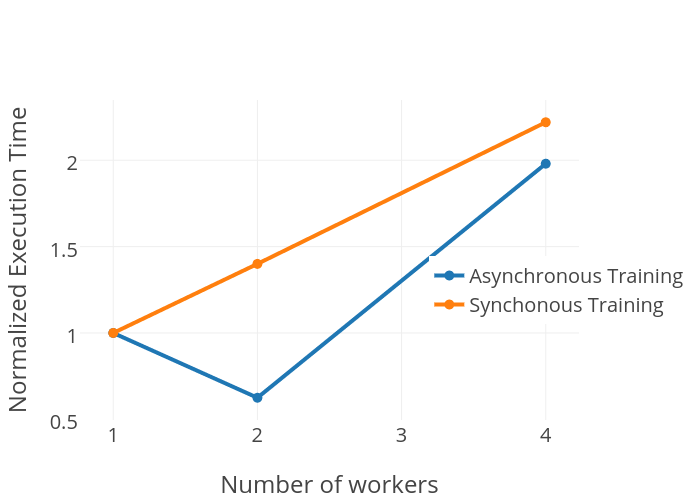
\includegraphics[keepaspectratio,width=.9\columnwidth]{figures/15712-corrected-scalability.png}
  \caption{\textbf{Scalability to multiple workers}}
  \label{fig:scalability}
\end{figure}

Figure \ref{fig:scalability} shows the execution time required 
to complete 20000 steps when run with 1,2 and 4 workers with
and without synchronization. The 
execution times for all the configurations are normalized to 
the single worker case. The data shows that the performance
of the precise and execution 





> Why distribute? 
Model parallelism allows training more complex models with many 
parameters. This is a progression from using GPUs to many different
machines. 

> synchronous training scalability. Impact of synchrony on accuracy
Why do we use synchronous training. Is it because we have a system
that is similar to the single node version? 
This berkeley thesis talks about why synchronization is important. 
Apparently synchronization allows for faster convergence because 
the average of the local updates of different machines reduces the
variance in data which leads to faster convergence. (https://www2.eecs.berkeley.edu/Pubs/TechRpts/2016/EECS-2016-47.pdf)
Blindly removing synchrony in an application does not seem to be
completely useful.

The impact of asynchrony on accuracy is that we are making judgements
on only part of the data that was present in our local store. This
higlights the dependence of the distribution of data and the homogeniety
(in terms of information) of the data. I think this was the premise of 
the hogwild paper.

> How does asynchrony affect training time? And accuracy
Stragglers are an issue in any large scale distributed training. If 
we use machines with different processing times (as in a distributed
cluster with different processing times) then the effects of stragglers
are exaggerated. 





\section{The Proposal}


In summary, our two primary goals in order to improve perfor- mance/energy efficiency are:
• Reducing coherence misses
• Reducing the amount of coherence traffic
In the case of computing with approximable data, we can allow the usage of data that does not necessarily have the latest value. This would enable us to (i) drop writebacks and invalidates to memory and other cores during processor writes and (ii) execute on imprecise stale data in the case of a processor read.
Ignoring all coherence messages for shared data would lead to a highly approximate and imprecise system. We, however, need to limit this imprecision by enabling coherence messages in such a manner so as to obtain an acceptable trade-off between precision and performance.

In this section, we describe our proposed approximate protocol. The key observation behind our proposed idea is that all updates are not equal. In fact, some writes make a huge difference while other slightly modify the previous data. As a result, we could treat them differently. It means that when there are only a small updates to the cache line, we might be able to avoid propagating those writes to other threads and eliminate the coherence messages plus avoid potential coherence misses.

The coherence traffic and coherence misses are mainly generated from transitions to the "Modified" state which results in invalidations to the same cachelines in other caches. In order to minimize these transi- tions, we propose to add another state to the cache coherence protocol to track modified data - "Highly Modified (H)" state. This state is treated in the same manner as a real modified state, where invalidates are sent to the directory and other caches and writebacks to DRAM are generated. The other modified state "Modified (M)" does not cause invalidations to data in the directory or other caches. In this case it is possible for a cacheline to exist simultaneously in the shared (S) and modified (M) states. The modified state primarily exists to control the transition from "H" and "M" and control impreci- sion. Upon eviction of data from the cache, data in the "M" state is still written back to memory as usual.

Figure 5 shows our proposed approximate cache coherence protocol. As it is shown in figure 5, when a big update reaches cache controller, it is treated as a regular write. It means that the cache line makes a transition to the H state and invalidate all other copies. Those copies could be in modified, shared or exclusive state. When a small updates gets to the cache controller, it simply makes a transition to the modified state.  



\begin{figure}[h]
  \centering
  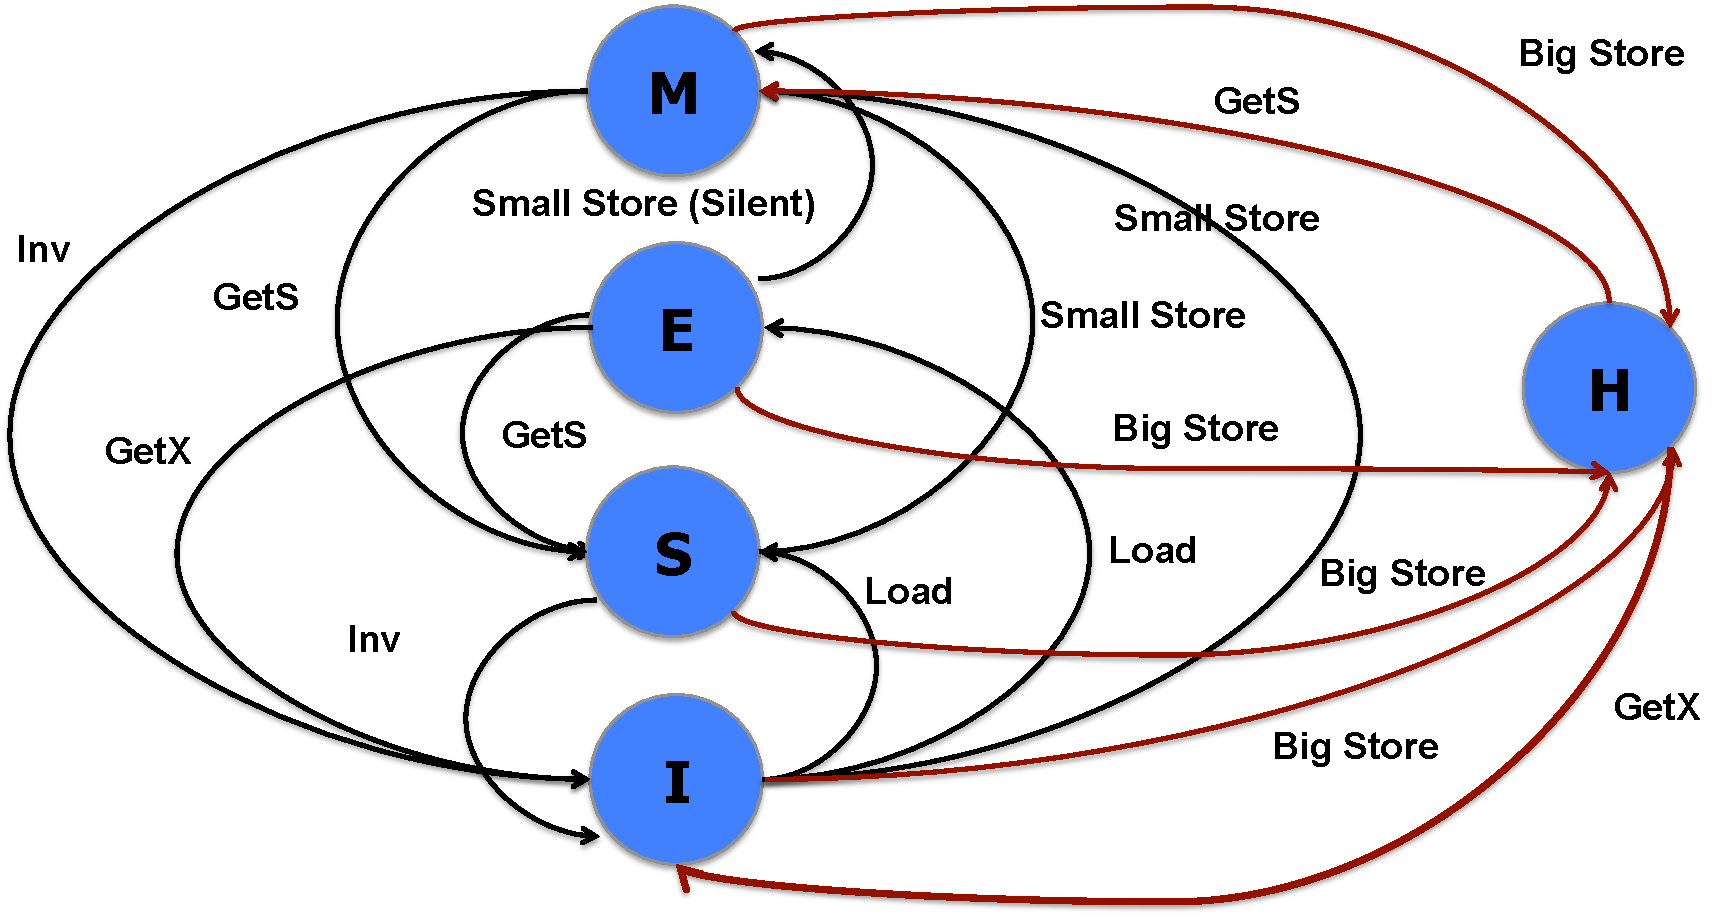
\includegraphics[height=2.5 in, width=3.2in]{figures/figure5.pdf}
  \caption{Approximate Coherence Protocol}
  \label{fig:profile}
\end{figure}


\section{Error Bounding}

An important challenge with an approximate coherence protocol is error bounding.
All forms of approximation at any level of the stack requires some mechanism to
ensure that the imprecision introduced into the system doesn't cause
catastrophic crashes to the system and provides a weak guarantee with respect
to the error bound specified by the programmer. We discuss a few mechanisms to
provide some sort of guarantee to the programmer. The error bounding mechanism
here is essentially defining when an update is either "Big" or "Small". 

\subsection{Data-driven Error Bounding}  
Here, defining whether an update is "Big" or "Small" is defined by the size of
the update in terms of the data value. If the size falls within a predetermined
error threshold, it is treated as a "Small" update. Otherwise it is treated like
a "Big" Update. The tricky part here is conveying the threshold from what is 
desired by the programmer to the hardware, so we can make this decision. Also we
would need hardware to compare each data value during an update to determine how
"Big" or "Small" it is. This can lead to high overhead. 

\subsection{Probability Error Bounding}  
We can also switch between "Big" and "Small" updates \emph{probabilistically}.
This has high overhead since we no longer consider the data value itself and
seems use heuristics to determine the weight of the update. Some heuristics
could include: 
\begin{itemize}
\item Switch from "M" to "H" after a certain number of updates to a cache line.
\item Choose from "M" and "H" based on the number of cores that are sharing the
cache line
\item Choose form "M" and "H" is a globally probabilistic way.

\end{itemize}

\section{Methodology}
\label{sec:methodology}
\subsection{Infrastructure}
We use PIN to perform our primary design analysis. PIN is dynamic binary instrumentation tool for
x86 architecture that collects runtime information by inserting extra code into
the program. PIN enables a much
faster evaluation without the full architecutural simulation. Since Gem5 is too
heavy-weight for initial experimentation, we built a
cache model with flexible coherence support using PIN. We added the "H" state
to our MESI-based cache simulator. We measure the difference in coherence
misses, invalidate/write back traffic and directory lookups to determine the
impact of the MESHI protocol. 

\begin{table}
  \centering
  \begin{tabular}{||c|c||}
	\hline
	
	\multicolumn{2}{||c||}{\textbf{Cache Hierarchy}} \\
	\hline
	L1 D-cache & 64KB/4 way, 64B block size\\ \hline
	Coherence Protocol & MESI Directory-based \\
	\hline

  \end{tabular}
  \caption{Simulator Parameters}
  \label{table:sim_param}		

\end{table}
\subsection{Assumptions and Simplifications}
We simply allow the approximate protocol to impact the cache performance for the
workloads in our evaluation. Impacting the correctness and precision of the
program as a result of our approximate cache protocol is beyond the scope of
this project. Since we cannot measure the impact on precision of the program, we
simply vary the \emph{degree of approximation} as opposed to implementing any
specific error bounding mechanism described above. We vary the degree of
approximation by controlling the fraction of writes that are treated as "Big" as
opposed to "Small" by the cache coherence protocol. The is entirely
probabilistic and does not depend on the data within the cache line, nor the
number of updates to any particular cache line. In that sense, the results
below depict the worst case. We believe that more intelligent "Big" vs "Small"
prediction mechanisms are likely to lead to better results. We, however, leave
this evaluation as part of future work. 

\subsection{Workloads}
We use a subset of benchmarks from the PARSEC-2.1 suite - namely
\emph{streamcluster, bodytrack, vips, fluidanimate, canneal}. We picked
benchmarks that showed the highest amount of data sharing with short running
times. We used the \emph{simmedium} input set for our evaluation. We programmed
our simulator to collect data within the Region of Interests within each
benchmark and assume that all data touched within the ROI to be approximable.




\section{Results}
\label{sec:results}
\subsection{Coherence Misses}
Figure~\ref{fig:coherence} depicts the reduction in coherence misses with the
MESHI protocol. The coherence misses include both: (1) Loads to data found in
the \emph{INV} state in the cache and (2) Stores to data found in the cache in a
shared or invalid state. As expected, as the amount of approximation increases the coherence miss
count reduces. What is interesting is that in most cases the drop in coherence
misses is disproportionate with the fraction of "Big" writes. For example,
treating 20\% of all writes as "Big" reduces the number of coherence misses by
close to 97\% in most of the workloads that we evaluate here. The 25\% point in
\emph{streamcluster} seems to be an anomaly here.  
\begin{figure}[t] \centering 
%\vspace{-0.4cm}
%\vspace{-0.1cm}
\centering
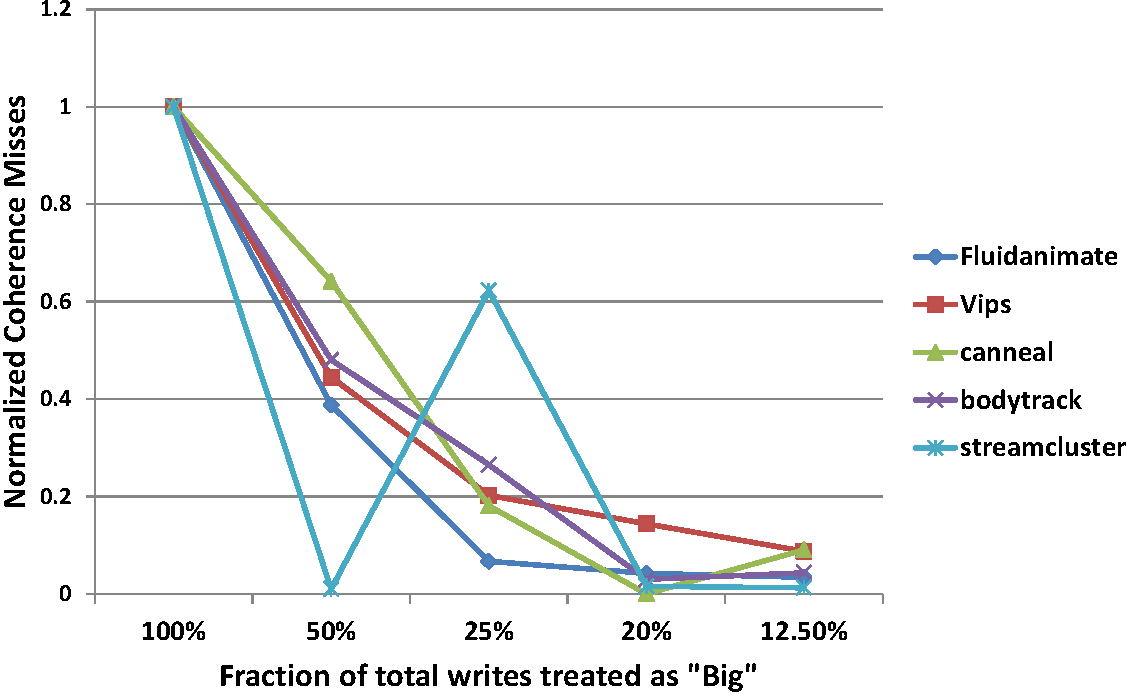
\includegraphics[width=0.49\textwidth]{figures/coherence_misses-crop.pdf}
\caption{Reduction in Coherence Misses.}
\label{fig:coherence}
\end{figure}

\subsection{Invalidate Traffic}
Figure~\ref{fig:invalidates} depicts the change in invalidate traffic as a
result of the approximate coherence protocol. We define the number of
invalidates the number of messages to other caches to invalidate cache lines
because of the cache coherence protocol. We observe the impact of
approximation varies across different workloads. For example, \emph{bodytrack}
benefits the least, with the reduction in invalidate traffic being only about
20\% even with aggressive approximation. Whereas \emph{vips} benefits a lot
more commensurately with the approximation. We attribute this difference to the
amount of sharing between different threads at any given time, where \emph{vips}
most likely has a lot more cores sharing a piece of data during an write
operation than \emph{bodytrack}.  

\begin{figure}[t] \centering 
%\vspace{-0.4cm}
%\vspace{-0.1cm}
\centering
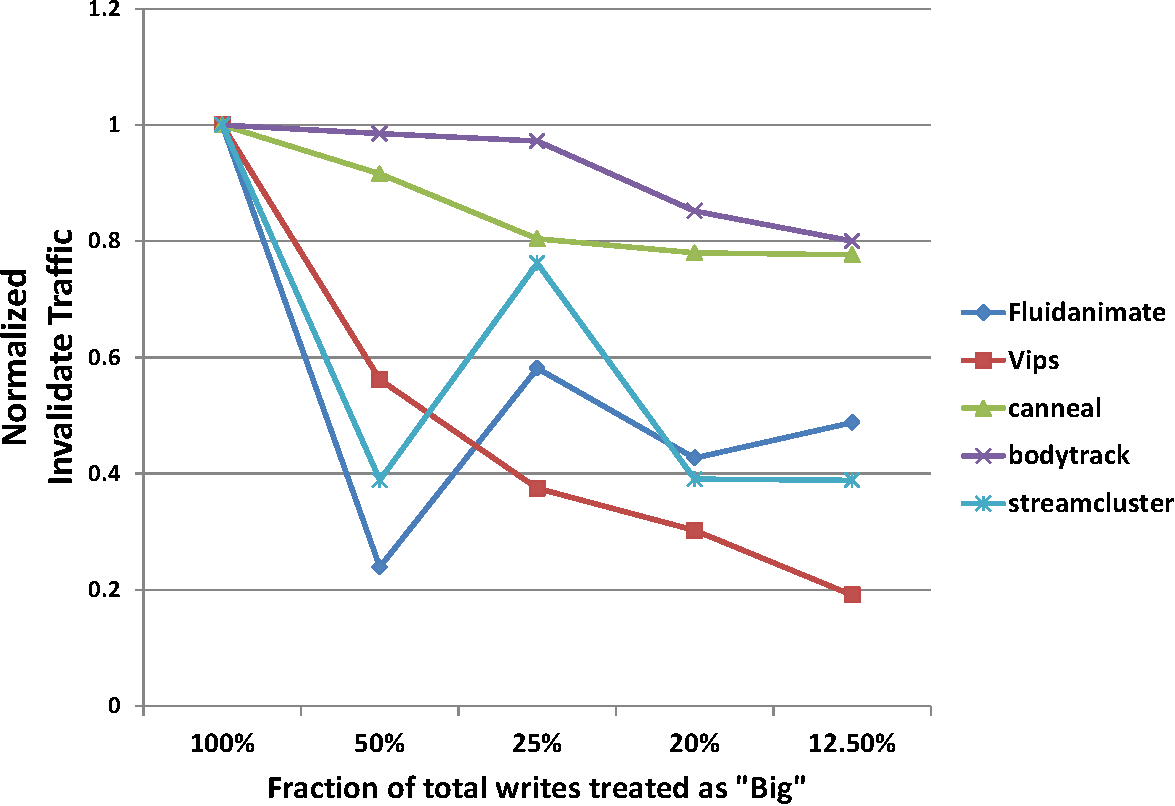
\includegraphics[width=0.49\textwidth]{figures/Invalidates-crop.pdf}
\caption{Reduction in Invalidate Traffic.}
\label{fig:invalidates}
\end{figure}

\subsection{Directory Lookups}
Figure~\ref{fig:lookups} depicts the number of the directory lookups as we vary
the extent
of approximation in the coherence protocol. Again we see a huge drop in the
number of directory lookups at a certain point (20\%) in most of the workloads.
Upto that point the reduction is more on-par with the fraction of "Big" writes.
The "M" state allows for a lot more silent updates than before.  

\begin{figure}[t] \centering 
%\vspace{-0.4cm}
%\vspace{-0.1cm}
\centering
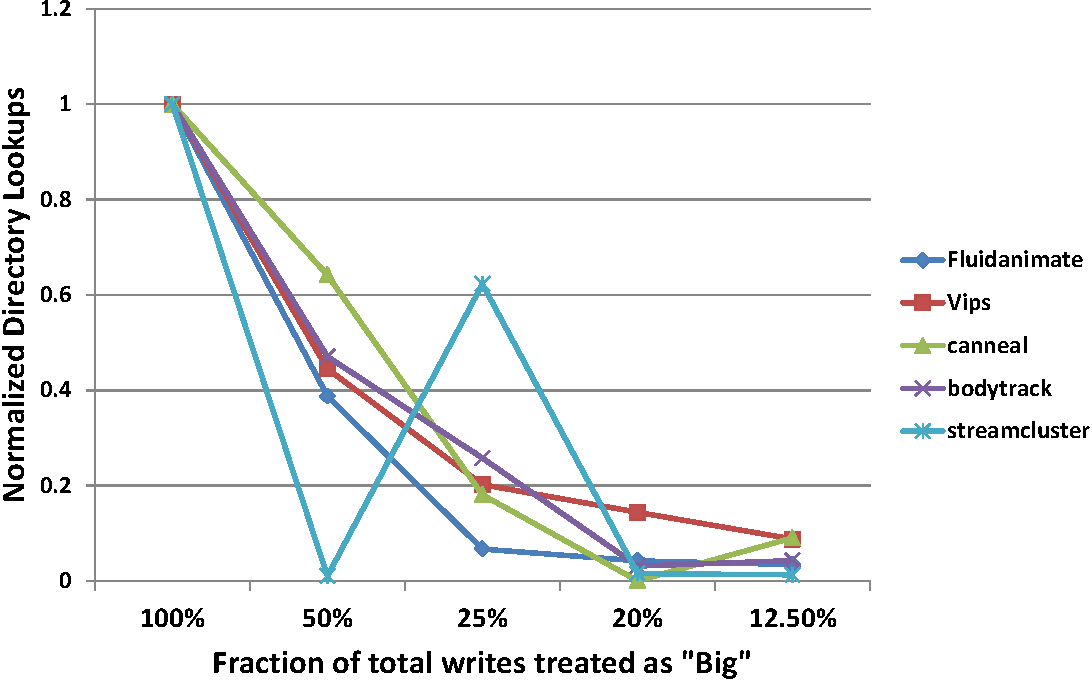
\includegraphics[width=0.49\textwidth]{figures/Lookups-crop.pdf}
\caption{Reduction in Directory Lookups.}
\label{fig:lookups}
\end{figure}

\subsection{Writebacks}
Figure~\ref{fig:writeupdates} shows the number of cache lines that were shuttled
back and forth across cores as a result of data sharing. As expected,
approximation certainly provides a reduction in the number of cache lines that
ping-pong between different cores. The extent again varies across the different
workloads, with \emph{Canneal} and \emph{Bodytrack} benefitting the most.  
 
\begin{figure}[t] \centering 
%\vspace{-0.4cm}
%\vspace{-0.1cm}
\centering
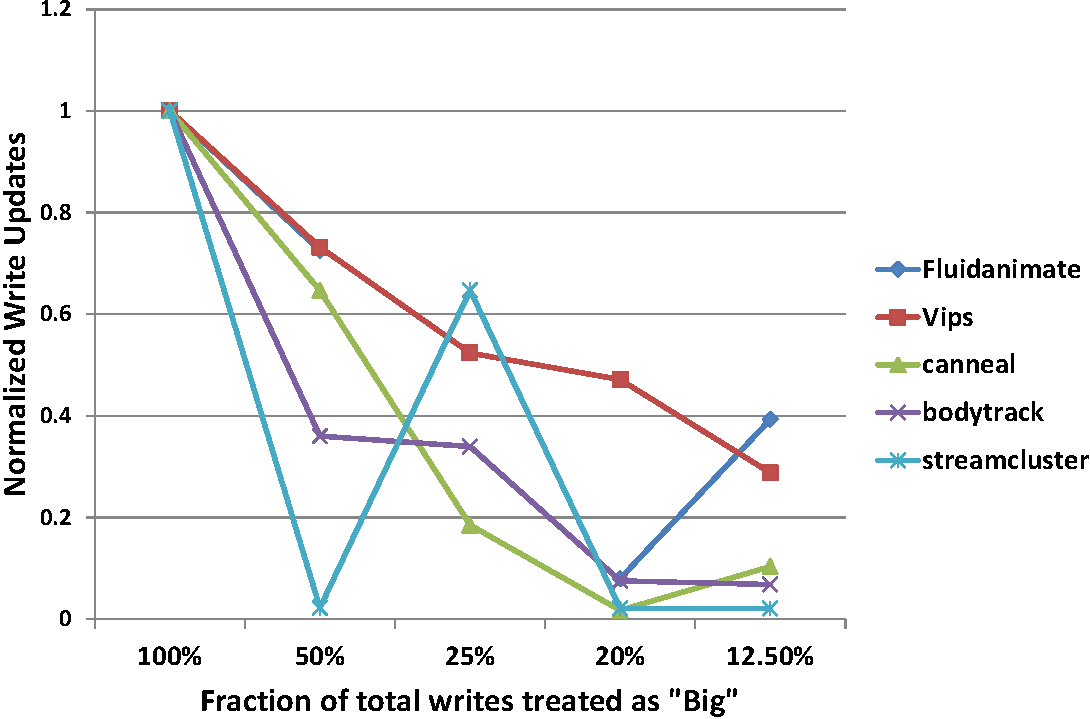
\includegraphics[width=0.49\textwidth]{figures/WriteUpdates-crop.pdf}
\caption{Reduction in Writebacks.}
\label{fig:writeupdates}
\end{figure}


\section{Conclusion}
\subsection{Learnings:}
\subsection{Contributions:}
\begin{itemize}
\item An analysis of the scalability of distributed training using TensorFlow
\item An evaluation of heterogeneous approximation techniques to accelerate distributed training
\end{itemize}
\subsection{Constraints:}

%\section{Future Work}


\bstctlcite{bstctl:etal, bstctl:nodash, bstctl:simpurl}
\bibliographystyle{IEEEtranS}
\bibliography{references}

\end{document}

